%\maketitle

\tableofcontents

\newpage

\section{Задание}
По выданному преподавателем варианту восстановить текст заданного варианта программы и подпрограммы (программного комплекса), определить предназначение и составить его описание, определить область представления и область допустимых значений исходных данных и результата, выполнить трассировку программного комплекса.

\begin{figure}[H]
\centering
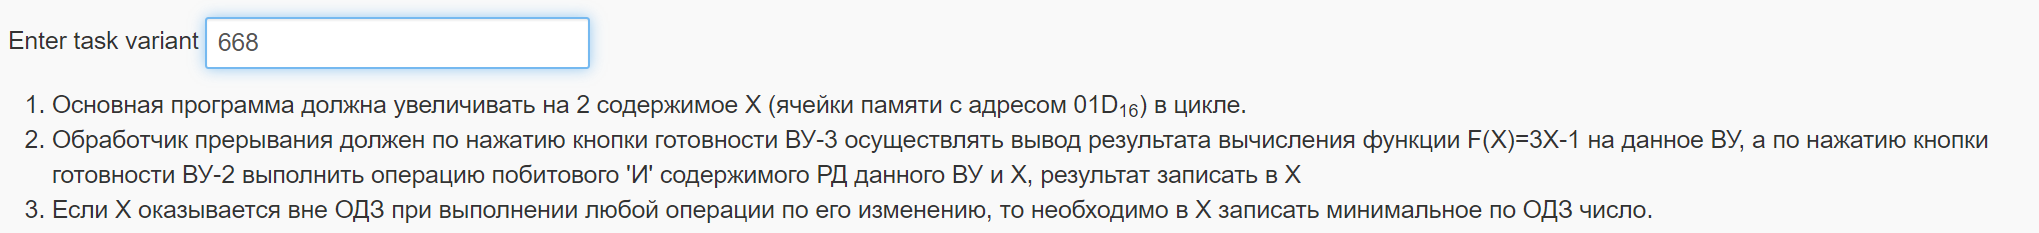
\includegraphics[scale=0.6]{task}
\label{pic:task}
\end{figure}


\section{Текст программы}
\subsection{Основная программа}
\begin{center}
	\begin{tabular}{|c|c|c|l|}
		\hline
		\textbf{Адрес ячейки} & \textbf{Содержимое ячейки} & \textbf{Мнемоника} & \textbf{Комментарии}\\
		\hline
		3B8 & 0200 & CLA & Очистка аккумулятора \\
		3B9 & EE18 & ST IP + 24 & Сохраненине 0 в ячейку 0x3D2 \\
		\hline
		3BA & AE14 & LD IP + 20 & Загрузка в AC содержимого из ячейки 0x3CF \\
		3BB & 0C00 & PUSH & Запись AC в стек \\
		3BC & D6DB & CALL \$6DB & Вызов подпрограммы по адресу 0x6DB \\
		3BD & 0800 & POP & Чтение из стека в AC \\
		3BE & 0740 & DEC & Декремент AC \\
		3BF & 4E12 & ADD IP + 18 & Сложение AC с содержимым ячейки 0x3D2 \\
		3C0 & EE11 & ST IP + 17 & Сохраненине AC в ячейку 0x3D2 \\
		\hline
		3C1 & AE0E & LD IP + 14 & Загрузка в AC содержимого из ячейки 0x3D0 \\
		3C2 & 0C00 & PUSH & Запись AC в стек \\
		3C3 & D6DB & CALL \$6DB & Вызов подпрограммы по адресу 0x6DB \\
		3C4 & 0800 & POP & Чтение из стека в AC \\
		3C5 & 6E0C & SUB IP + 12 & Вычитание из AC содержимого ячейки 0x3D2 \\
		3C6 & EE0B & ST IP + 11 & Сохранение AC в ячейку 0x3D2 \\
		\hline
		3C7 & AE09 & LD IP + 9 & Загрузка в AC содержимого ячейки 0x3D1 \\
		3C8 & 0C00 & PUSH & Запись AC в стек \\
		3C9 & D6DB & CALL \$6DB & Вызов подпрограммы по адресу 0x6DB \\
		3CA & 0800 & POP & Чтение из стека в AC \\
		3CB & 0700 & INC & Инкремент AC \\
		3CC & 4E05 & ADD IP + 5 & Сложение AC с содержимым ячейки 0x3D2 \\
		3CD & EE04 & ST IP + 4 & Сохранение AC в ячейку 0x3D2 \\
		3CE & 0100 & HLT & Остановка ТГ \\
		\hline
		3CF & ZZZZ & Z & Первый аргумент \\
		3D0 & YYYY & Y & Второй аргумент \\
		3D1 & XXXX & X & Третий аргумент \\
		3D2 & 0028 & R & Результат \\
		\hline
	\end{tabular}
\end{center}

\newpage




\subsection{Подпрограмма}
\begin{center}
	\begin{tabular}{|c|c|c|l|}
		\hline
		\textbf{Адрес ячейки} & \textbf{Содержимое ячейки} & \textbf{Мнемоника} & \textbf{Комментарии}\\
		\hline
		6DB & AC01 & LD \&1 & Чтение из стека входного параметра \\
		6DC & F204 & BMI IP + 4 & Если значение параметра меньше нуля,\\
		& & & то переход в ячейку 0x6E1 \\
		6DD & F003 & BEQ IP + 3 & Если значение параметра равно нулю, \\
		& & &то переход в ячейку 0x6E1 \\
		6DE & 7E0A & CMP IP + 10 & Сравнение AC с содержимым ячейки 0x6E9 \\
		6DF & F006 & BEQ IP + 6 & Если значение параметра равно содержимому\\
		&&&  ячейки 0x6E9, то переход в ячейку 0x6E6 \\
		6E0 & F805 & BLT IP + 5 & Если значение параметра меньше содержимого\\
		&&& ячейки 0x6E9, то переход в ячейку 0x6E6 \\
		6E1 & 0500 & ASL & Арифметический сдвиг влево \\
		6E2 & 0500 & ASL & Арифметический сдвиг влево \\
		6E3 & 6С01 & SUB \&1 & Вычитание из AC входного параметра \\
		6E4 & 4E05 & ADD IP + 5 & Сложение с AC сожержимого ячейки 0x6EA \\
		6E5 & CE01 & BR IP + 1 & Безусловный переход в ячейку 0x6E7 \\
		6E6 & AE02 & LD IP + 2 & Загрузка в AC содержимого ячейки 0x6E9\\
		6E7 & EC01 & ST \&1 & Сохранение AC на место входного \\
		&&&параметра в стеке \\
		6E8 & 0A00 & RET & Возврат из подпрограммы \\
		\hline
		6E9 & 0D2F & a & Локальная переменная \\
		6EA & 0026 & b & Локальная переменная \\
		\hline
		
	\end{tabular}
\end{center}

\section{Описание программы}
\subsection{Назначение программы и реализуемая ею функция}
\subsubsection{Реализуемая программой функция}
	\begin{center}
		$ R = F(X) + F(Y) - F(Z) + 2 $
	\end{center}
\subsubsection{Реализуемая подпрограммой функция}
	\begin{center}
		\[
			F(x) =  \begin{cases}
			3x + b & \textrm{, для } x\leq0\textrm{,}\\
			a & \textrm{, для } 0<x\leq a\textrm{,}\\
			3x + b & \textrm{, для } x>a
			\end{cases}
		\]
	\end{center}

\subsubsection{График функции, реализуемый подпрограммой}
\begin{figure}[H]
	\centering
	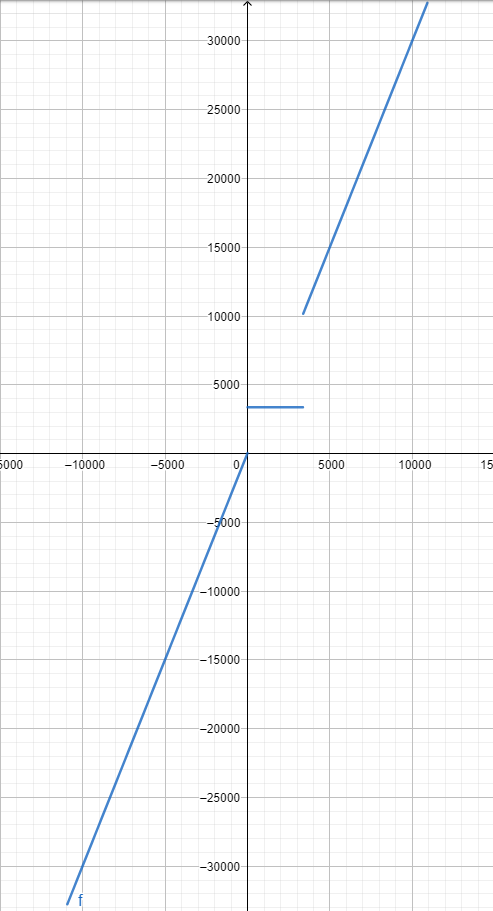
\includegraphics[scale=0.5]{graphic}
	\label{pic:graphic}
\end{figure}

\subsection{Область представления и область допустимых значений исходных данных и результата}
\subsubsection{Область представления}
\noindent Z, Y, X, R - 16-разрядные знаковые числа с фиксированной запятой. Диапазон значений формата: $-2^{15}\ldots2^{15}-1$\\


\subsubsection{Область допустимых значений}
\noindent Область допустимых значений R совпадает с областью представления.\\
\\
Область допустимых значений входного аргумента подпрограммы (т.е. $ X,Y,Z $):\\
\hspace*{1cm} Пусть $ F(x) $ - реализуемая подпрограммой функция, тогда ОДЗ для нее будет $-2^{15}\ldots2^{15}-1$.\\
\\
\hspace*{1cm} 1) Пусть $ -32768 \leq x\leq0 $, тогда имеет место система:
\[
	\begin{cases}
	 -32768 \leq F(x) \leq 32767 \\
	-98266\leq F(x)\leq 38\\
	\end{cases}
\]
\hspace*{1cm}Откуда $ F(x) = 3x + 38 \geq -32768 \Rightarrow x \geq -10935$\\
\hspace*{1cm}В итоге \[
	\begin{cases}
	-10935 \leq x \leq 0\\
	-32768 \leq F(x) \leq 38
	\end{cases}
\]
\\
\hspace*{1cm} 2) Пусть $ -0<x\leq a $, тогда $ F(x) = a $\\
\\
\hspace*{1cm} 3) Пусть $ a <x\leq 32767 $, тогда имеет место система:
\[
\begin{cases}
-32768 \leq F(x) \leq 32767 \\
10163\leq F(x)\leq 98339\\
\end{cases}
\]
\hspace*{1cm}Откуда $ F(x) = 3x + 38 \leq 32767 \Rightarrow x \leq 10909$\\
\hspace*{1cm}В итоге \[
\begin{cases}
3375 \leq x \leq 10909\\
10163 \leq F(x) \leq 32767
\end{cases}
\]

В итоге ОДЗ для $ X,Y,Z $ будет $  -10935 \leq x \leq 10909 $



\subsection{Расположение в памяти ЭВМ программы, исходных данных и результатов}
\subsubsection{Исходные данные и результат}
\noindent Z (0x3CF) - первый аргумент\\
Y (0x3D0) - второй аргумент\\
X (0x3D1) - третий аргумент\\
R (0x3D2) - результат выполнения программы\\
\subsubsection{Программа}
\noindent 0x3B8 --- 0x3CE - основная программа\\
0x6DB --- 0x6E8 - подпрограмма\\
a (0x6E9), b (0x6EA) - локальные переменные, используемые подпрограммой


\subsection{Адреса первой и последней выполняемой команд программы}
\noindent 0x3B8 - первая исполняемая команда программы\\
0x3CE - последняя исполняемая команды программы\\

\newpage
\section{Таблица трассировки}
\begin{center}
	\begin{tabular}{|c|c|c|c|c|c|c|c|c|c|c|c|}
		\hline
		\multicolumn{2}{|c}{\makecell{\textbf{Выполняемая}\\\textbf{команда}}}
		&\multicolumn{8}{|c|}{\textbf{Содердимое регистров после выполнения команды}}
		&\multicolumn{2}{c|}{\makecell{\textbf{Ячейка, содержимое}\\\textbf{которой изменилось}}}\\
		\hline
		Адрес & Код & IP & CR & AR & DR & SP & BR & AC & NZVC & Адрес & Новый код\\
		\hline
	\end{tabular}
\end{center}
\newpage

\section{Вывод}
\noindent В ходе выполнения данной лабораторной работы я познакомился с реализаций стека в БЭВМ и впервые им пользовался. Также я научился работать с подпрограммами и узнал какими способами можно передавать аргументы в подпрограммы.